\section{方法：GAST 预测框架}
\label{sec:method}

\subsection{总体结构与设计原则}

GAST 由带掩码的历史编码器与目标条件化的多模态解码器组成。其组织方式源于一个决定：有效性掩码不是与坐标并列的输入通道，而是显式的\emph{观测证据状态}的生成依据，后续每一级都读取该状态。由此得到三条设计原则。

\textbf{P1：证据具有层级性而非局部性。}一帧是否可信取决于该行人距上次被观测已过多久，因此证据状态是缺失年龄的函数，并由各模块共享，而不是由每个模块各自重新计算。

\textbf{P2：未观测行人可以“听”，但不能“说”。}当前未被观测的行人仍可借助邻居被预测，但其陈旧位置不得作为当前证据提供给其他行人。该不对称性在关系注意力中被强制执行。

\textbf{P3：解码从证据结束处开始。}预测起点可能晚于最后一次观测若干帧。解码器以最后观测位置为锚点，并被显式告知经过的间隔，使其首个预测点与（未知的）未观测区间保持一致，而不是被固定在一个占位行上。

图~\ref{fig:arch} 给出整体结构。编码器由逐帧关系编码（GERE）与证据条件化因果时间聚合（ECTA）两部分组成；解码器为 $K=20$ 个模式分别预测相对锚点的终点，并在该终点条件下生成残差轨迹。任何阶段都不接收插补坐标。

\begin{figure*}[t]
\centering
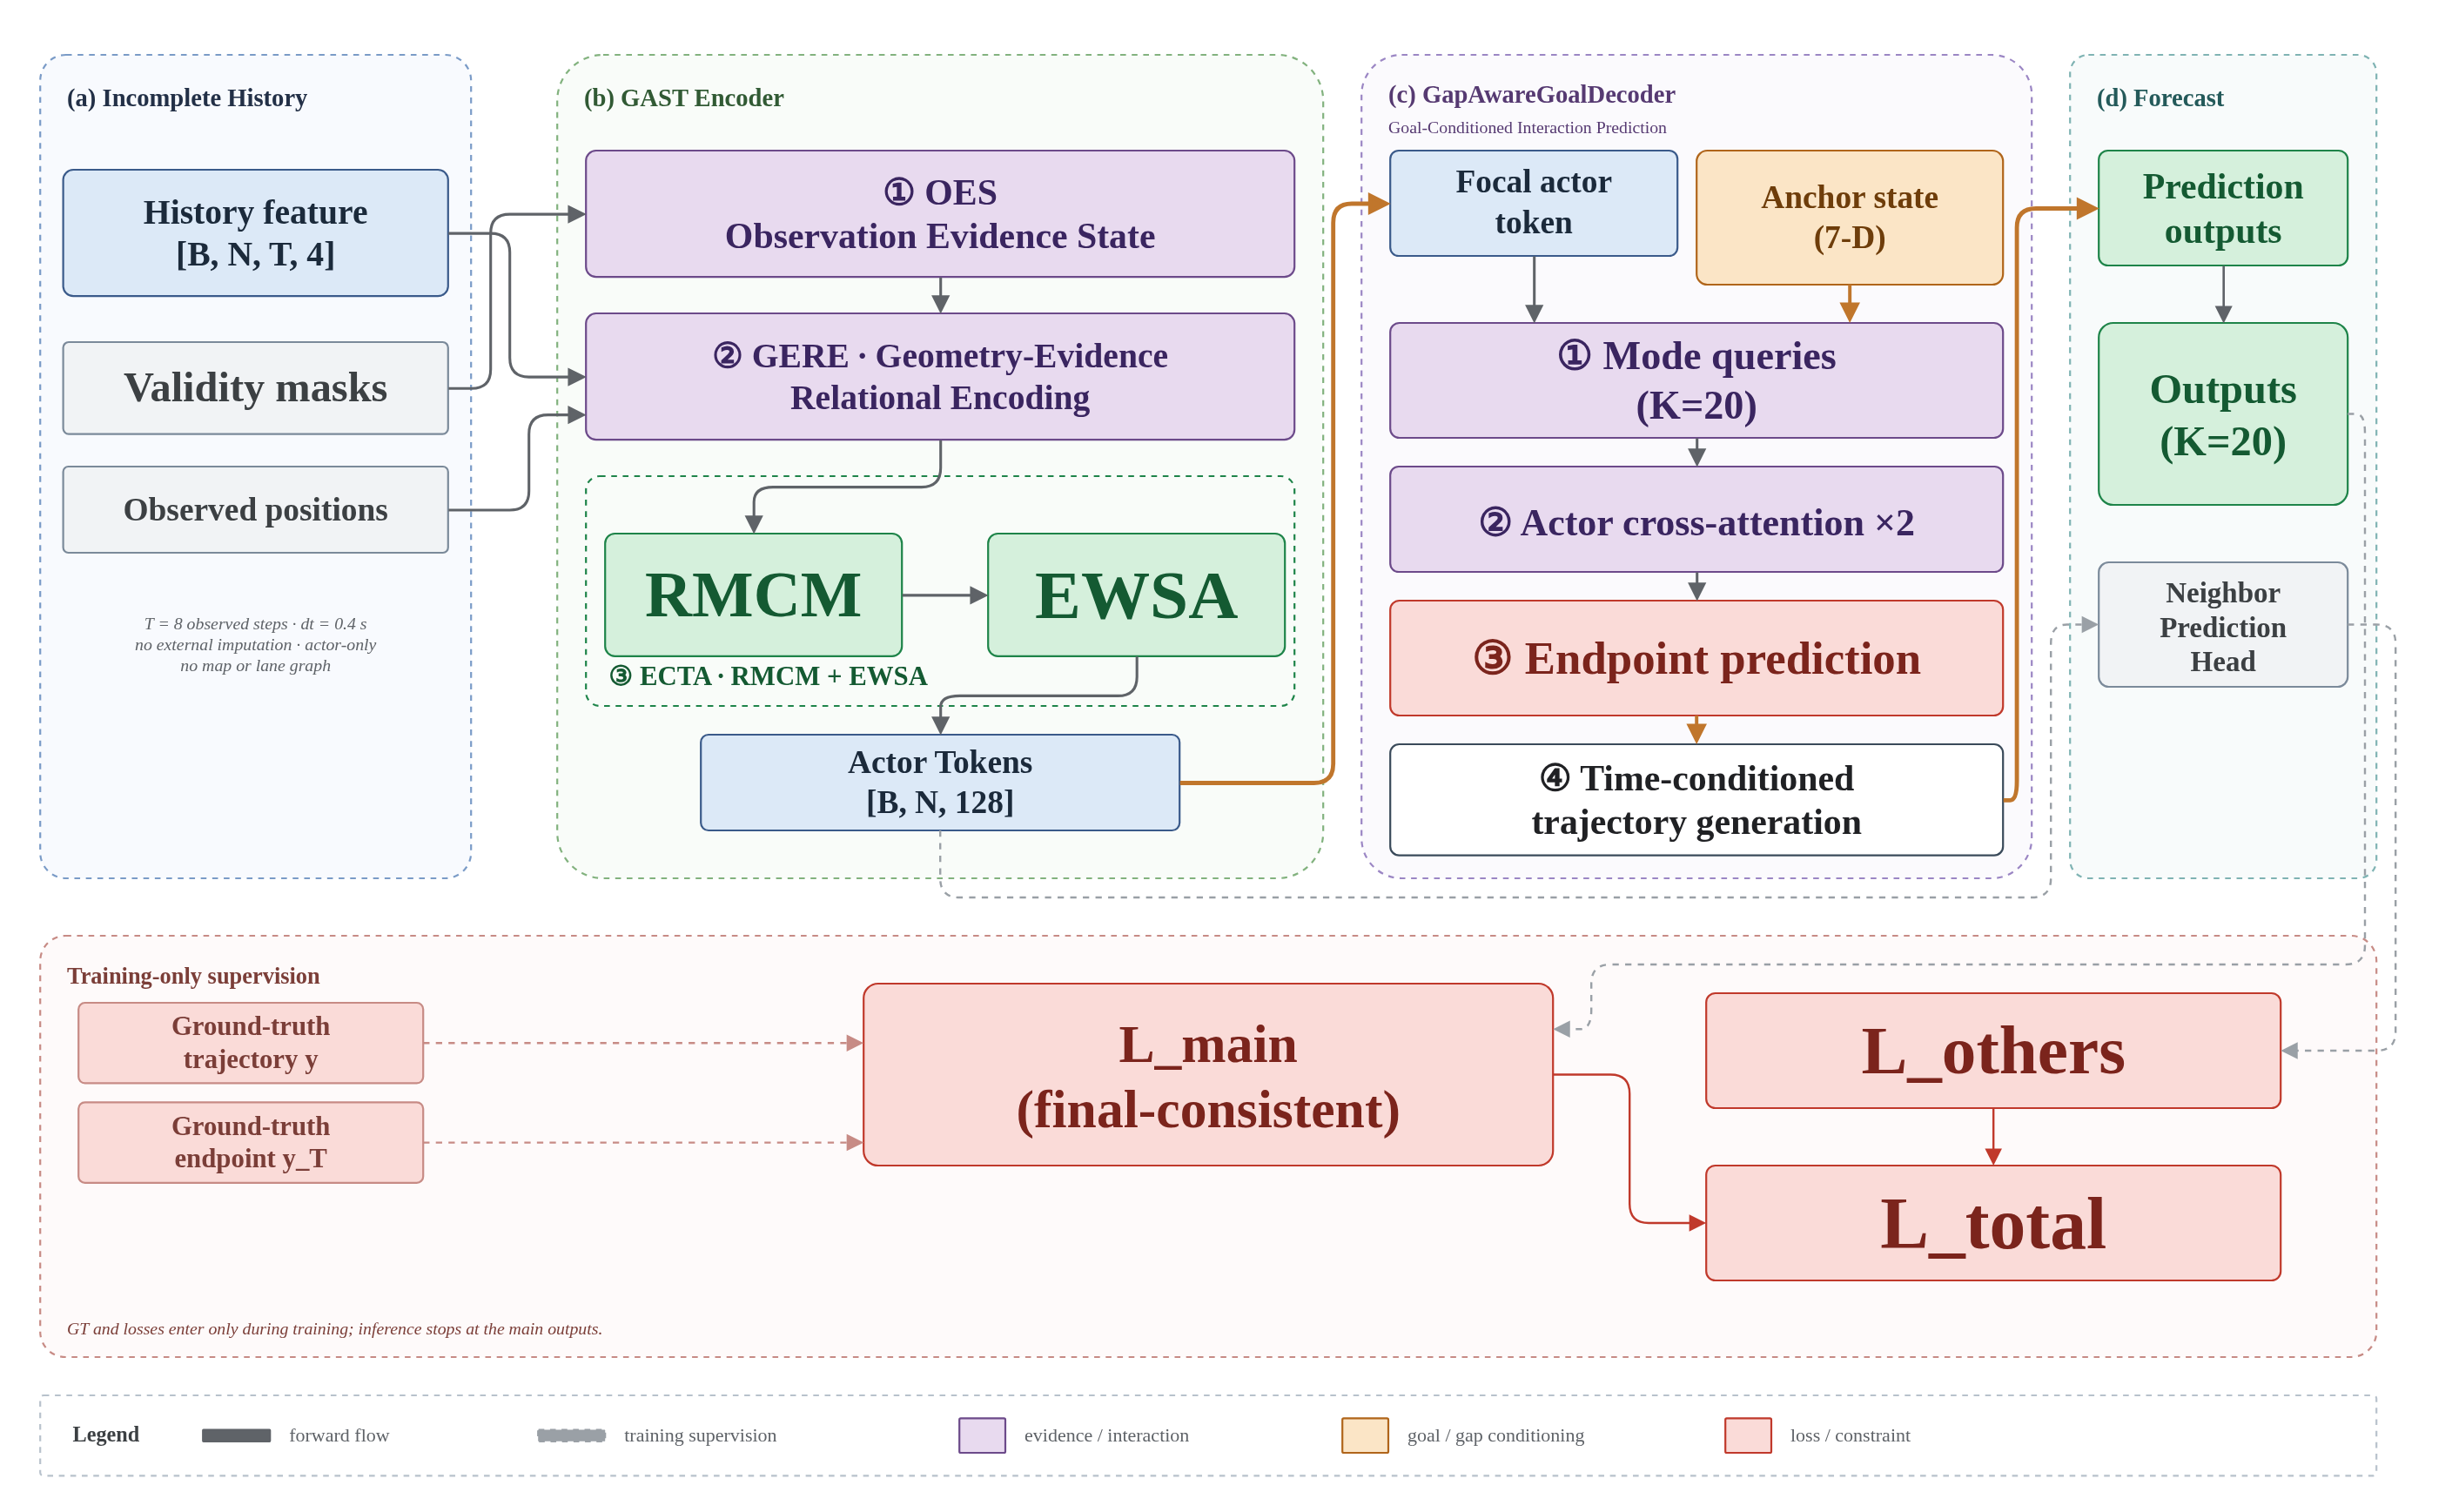
\includegraphics[width=0.94\textwidth]{figures/architecture_crop.png}
\caption{GAST 整体结构。(a) 带掩码的历史仅由位置、有效性掩码与观测位置表示，缺失项为占位值；(b) 观测证据状态（OES）驱动 GERE 与 ECTA，前者执行带几何偏置与源资格约束的逐帧关系注意力，后者按证据强度缩放时间输入（RMCM）并以证据加权方式聚合状态（EWSA）；(c) 目标条件化解码器由最后观测帧构造七维锚点状态（Anchor State），形成 $K$ 个模式查询，并为每个模式预测终点与随进度衰减的残差；(d) 输出 $K$ 条带概率与逐模式尺度的轨迹，邻居预测头仅在训练阶段使用。}
\label{fig:arch}
\end{figure*}

\subsection{观测证据状态}
\label{sec:oes}

对行人 $i$ 与历史步 $t$，记
\begin{equation}
a_{i,t}=t-\max\{t'\le t: m_{i,t'}=1\},
\label{eq:age}
\end{equation}
为距最近一次观测的年龄；当 $t$ 之前不存在有效观测时取 $a_{i,t}=t$（相当于假定窗口之前存在一次虚拟观测）。该状态包含三个量：资格 $s_{i,t}=m_{i,t}$，用于判定该帧能否作为证据来源；年龄 $a_{i,t}$；以及可靠度
\begin{equation}
r_{i,t}=m_{i,t}+(1-m_{i,t})\,\exp(-\tau\,a_{i,t}),\quad \tau=\mathrm{softplus}(\vartheta),
\label{eq:reliability}
\end{equation}
其中 $\vartheta$ 为单一可学习标量，初始化使其满足 $\tau\approx0.1$。可靠度在观测帧上恰为 1，在缺口内单调衰减。填充行的状态被排除，其 $r$ 置零。

式~\eqref{eq:reliability} 有两个性质值得强调。第一，它不是标定后的概率，本文也从不将其解释为概率：它是任务内部的可靠度变量，作用是按证据支持度为历史状态排序。第二，它在完整历史上为恒等映射（$r\equiv1$），此时证据条件化消失，GAST 退化为其骨干网络。这使本文模型能够在无分布偏移的前提下与完整历史结构进行比较。

\subsection{GERE：带几何偏置的逐帧关系编码}
\label{sec:gere}

行人 $i$ 在每一帧的输入为四维向量
\begin{equation}
u_{i,t}=\big[\Delta p_{i,t},\ \Delta s_{i,t},\ m_{i,t}\big],
\label{eq:input}
\end{equation}
分别对应位置增量、观测速度增量与有效性标记，经 patch 嵌入得到 $h_{i,t}=\mathrm{PatchEmbed}(u_{i,t})$。

\textbf{幽灵标记。}每一帧把整个场景的有效性模式池化为一个标记：
\begin{equation}
g_{t}=\mathrm{max}_{i\in\mathcal{V}_{t}}\ \psi\big(\mathbf{1}-m_{i,t}\big),
\label{eq:ghost}
\end{equation}
其中 $\psi$ 为作用于“标量掩码在通道维广播后”的两层嵌入，$\mathcal{V}_{t}$ 为非填充行人的集合。该标记沿用文献 \cite{xu2025sportstraj} 的逐帧空间编码设计，并将其适配到带掩码的历史。标记被前置到该帧的 $N$ 个行人标记之前参与注意力，计算后移除。由于其输入仅为掩码，幽灵标记概括了“当前谁可被观测”，不携带任何位置内容，因而不会注入虚假坐标；但它为所有行人提供了关于场景当前可观测性的共享描述。

\textbf{源资格。}注意力的键只允许取自幽灵标记与满足 $s_{j,t}=1$ 的行人；所有行人（包括未被观测者）仍是合法的查询。因此未被观测的行人可以读取邻居与场景摘要的当前状态，而其自身的陈旧特征不会被其他行人关注。这实现了 P2，也与“仅把掩码作为特征拼接”不同——后者会把陈旧标记留在键集合中。

\textbf{几何偏置。}对每个有序对 $(i,j)$，模型由观测几何构造七维关系描述子
\begin{equation}
f_{ij,t}=\big[\Delta p_{ij},\log(1+\|\Delta p_{ij}\|),\Delta v_{ij},\cos\Delta\theta_{ij},\sin\Delta\theta_{ij}\big],
\label{eq:geom}
\end{equation}
其中 $\Delta p_{ij}=p_{j,t}-p_{i,t}$，$\Delta v_{ij}=v_{j,t}-v_{i,t}$，$\Delta\theta_{ij}$ 为朝向角之差。速度由当前观测位置与前一\emph{有效}位置之差除以两者间的步数估计，因此缺口不会造成速度尖峰；若对中任一端未被观测，则 $f_{ij,t}=\mathbf{0}$。该描述子被映射为每个注意力头一个偏置，
\begin{equation}
B_{ij,t}^{(h)}=w_{2}^{(h)\top}\,\mathrm{GELU}\big(W_{1}f_{ij,t}\big),
\label{eq:bias}
\end{equation}
并加到行人—行人注意力块的 logits 上。式~\eqref{eq:bias} 的输出投影零初始化，因此训练从“无几何”的关系编码器出发，只有在该偏置确实降低目标函数时才被学习。关系编码逐帧进行，输出为每个行人的空间状态序列。

\subsection{ECTA：证据条件化因果时间聚合}
\label{sec:ecta}

\textbf{RMCM（可靠度调制的因果编码器）。}空间状态先经投影，再按可靠度缩放后进入因果递推：
\begin{equation}
\tilde{x}_{i,t}=\mathrm{MLP}(x_{i,t})\cdot r_{i,t},
\qquad
u_{i,1:T}=\mathrm{SSM}_{\phi}(\tilde{x}_{i,1:T}),
\label{eq:rmcm}
\end{equation}
其中 $\mathrm{SSM}_{\phi}$ 为四层单向选择性状态空间块 \cite{gu2023mamba}。因果性是必需的：预测不得依赖未来的历史位置，同时也使编码器可用于流式部署。调制是逐帧、通道共享的标量，改变的是状态进入递推的强度而非状态本身的含义。具体而言，观测帧以单位强度进入，而连续缺失三步的帧被 $e^{-3\tau}$ 衰减，从而难以用衰减后的状态覆盖最后一次可靠状态。

\textbf{EWSA（证据加权状态聚合）。}读出不再固定取最后一个时间步。以内容得分 $e_{i,t}=w^{\top}u_{i,t}$、温度 $\beta=1$，模型计算
\begin{equation}
\alpha_{i,t}=\mathrm{softmax}_{t}\big(e_{i,t}+\beta\log r_{i,t}\big),\qquad
\bar{h}_{i}=\sum_{t}\alpha_{i,t}\,u_{i,t},
\label{eq:ewsa}
\end{equation}
并以末端可靠度在末端状态与该聚合之间做门控：
\begin{equation}
z_{i}=r_{i,T}\,u_{i,T}+\big(1-r_{i,T}\big)\bar{h}_{i}.
\label{eq:gate}
\end{equation}
当末帧被观测时 $z_{i}=u_{i,T}$，读出与标准的末端读出完全一致；当末帧缺失时，模型回退到可用状态的加权平均，权重同时受学习到的内容得分与证据强度塑形。该门控在形式上是硬切换，在数值上是软过渡，因为 $r_{i,T}$ 随末端缺口连续衰减。

\subsection{锚点条件化目标解码}
\label{sec:decoder}

\textbf{锚点状态（Anchor State）。}设 $\ell_{i}$ 为最后一个有效观测帧的下标，$\ell'_{i}$ 为其前一个有效观测帧的下标。解码器接收
\begin{equation}
\varphi_{i}=\Big[p_{i,\ell_i},\ v_{i},\ \tfrac{\delta_{i}}{T},\ \rho_{i},\ \mathbb{1}[\ell_{i}<T]\Big]\in\mathbb{R}^{7},
\label{eq:anchor}
\end{equation}
其中 $\delta_{i}=T-\ell_{i}+1$ 为末次观测到预测起点的步数，$v_{i}=(p_{i,\ell_i}-p_{i,\ell'_i})/(\ell_i-\ell'_i)$ 为缺口感知速度（只有一帧观测时为零），$\rho_{i}=\frac{1}{T}\sum_{t}m_{i,t}$ 为有效观测比例，末项标记末端缺失。保留锚点位置分量是为使该模块在任意坐标系下有定义；在第~\ref{sec:task} 节的锚点中心化归一化下该分量恒为零，状态信息由速度与间隔描述子承载。

\textbf{模式查询。}由式~\eqref{eq:gate} 得到的行人表示 $z_{i}$ 与锚点嵌入 $e^{\varphi}_{i}=\mathrm{MLP}(\varphi_{i})$ 同可学习的逐模式嵌入 $e_{k}$ 相加，
\begin{equation}
q_{i,k}=z_{i}+e^{\varphi}_{i}+e_{k},\qquad k=1,\dots,K,
\label{eq:query}
\end{equation}
再由两层交叉注意力在场景的行人表示上细化，填充行被屏蔽。每个模式因此在其自身的锚点条件下读取上下文，而不是共享单一场景向量。

\textbf{终点与轨迹。}一个预测头把每个模式查询映射为相对锚点的位移，
\begin{equation}
\hat{y}_{i,k,H}=p_{i,\ell_i}+\Delta_{i,k},\qquad \Delta_{i,k}=\mathrm{MLP}(q_{i,k}).
\label{eq:endpoint}
\end{equation}
对第 $t=1,\dots,H$ 步，令 $\tau_{t}=\delta_{i}+t-1$ 为锚点时刻到该未来步的经过步数，$p_{t}=\tau_{t}/(\delta_{i}+H-1)$ 为锚点—终点区间上的相对进度。轨迹由直线骨架与衰减残差构成：
\begin{equation}
\hat{y}_{i,k,t}=p_{i,\ell_i}+p_{t}\Delta_{i,k}+(1-p_{t})\,g_{\psi}(q_{i,k},e(\Delta_{i,k}),e(\tau_{t}\Delta t)).
\label{eq:traj}
\end{equation}
该构造有三点后果。第一，首个预测点已沿骨架推进 $\delta_{i}/(\delta_{i}+H-1)$，因此较长的末端缺口不会被默认为“行人停留在最后观测位置”。第二，残差在预测初期拥有完整自由度，且在 $t=H$ 处严格为零，使输出终点与预测目标一致。第三，由于 $p_{t}$ 以实际间隔为单位定义，同一模块无需特例即可处理观测末帧与末端缺失样本。

\textbf{模式概率与尺度。}评分头读取模式查询、终点嵌入与逐步查询的均值，输出 logits，经 softmax 得到 $\pi_{i,k}$。另一并行的头输出逐步、逐轴的 Laplace 尺度 $\sigma_{i,k,t}=\mathrm{ELU}(\cdot)+1.0001$，供下文似然项使用；$\sigma$ 是预测分布的离散度参数，不是标定后的置信区间。

\subsection{训练目标}
\label{sec:loss}

监督施加于目标行人（每个场景样本的第 0 个位置）。对模式 $k$，计算平均位移 $d_{k}$ 与终点误差 $d^{\mathrm{end}}_{k}$，并定义联合误差 $J_{k}=d_{k}+\lambda_{e}d^{\mathrm{end}}_{k}$，取 $\lambda_{e}=1$。两个不同的模式被用于两个不同目的：回归模式 $k^{\ast}=\arg\min_{k}J_{k}$ 兼顾形状与目的地，分类目标 $k^{\dagger}=\arg\min_{k}d_{k}$ 仅由轨迹级误差定义。总损失为
\begin{equation}
\mathcal{L}=\mathcal{L}_{\mathrm{reg}}+\mathcal{L}_{\mathrm{cls}}
+\mathcal{L}_{\mathrm{NLL}}+\mathcal{L}_{\mathrm{end}}
+\lambda_{d}\mathcal{L}_{\mathrm{div}}+\mathcal{L}_{\mathrm{nbr}},
\label{eq:loss}
\end{equation}
其中 $\mathcal{L}_{\mathrm{reg}}=\mathrm{SmoothL1}(\hat{y}_{k^{\ast}},y)$，$\mathcal{L}_{\mathrm{cls}}=-\log\pi_{k^{\dagger}}$，$\mathcal{L}_{\mathrm{end}}=\mathrm{SmoothL1}(\hat{y}_{k^{\ast},H},y_{H})$，$\mathcal{L}_{\mathrm{nbr}}=\mathrm{SmoothL1}(\hat{y}^{\mathrm{nbr}},y^{\mathrm{nbr}})$，$\mathcal{L}_{\mathrm{div}}=\mathbb{E}_{k\ne l}[0.5-\|\hat{y}_{k,H}-\hat{y}_{l,H}\|]_{+}$ 为终点两两距离上的合页项；$\mathcal{L}_{\mathrm{NLL}}$ 为附录~\ref{app:loss} 详述的 Laplace 负对数似然。交叉熵使用标签平滑 $0.2$，多样性权重 $\lambda_{d}=0.05$，间隔为 $0.5$~m。似然项在轨迹最接近的模式上计算，形式为逐步、逐轴平均的 $\log(2\sigma)+|y-\hat{y}|/\sigma$，并与软目标交叉熵 $0.5\sum_{k}\tilde{\pi}_{k}\log\pi_{k}$ 组合，其中 $\tilde{\pi}$ 由负轨迹误差经温度 softmax 得到；该项用于标定离散度并柔和地塑造模式分布，而不与硬分类目标竞争。邻居项由其他行人的编码状态预测其未来，仅在训练阶段生效；推理阶段模型只返回目标行人的 $K$ 条候选轨迹及其概率。

将 $k^{\ast}$ 与 $k^{\dagger}$ 分离是有意为之。概率应当按“模式对整条轨迹的解释程度”排序，而终点头应当在最符合目的地的模式上训练。若共用同一指派，必有一个目标被迫让步；分离二者在推理阶段不带来任何额外代价。

\subsection{性质}

\textbf{精确退化。}当所有 $m_{i,t}=1$ 时，式~\eqref{eq:reliability} 给出 $r\equiv1$：式~\eqref{eq:rmcm} 退化为普通因果编码器，式~\eqref{eq:gate} 返回末端状态，锚点状态仅承载观测速度，且 $\delta=1$、$\rho=1$、无末端缺失标记。此时缺失专用机制不产生任何作用，与完整历史基线之间的差异可归因于解码器与始终存在的场景级标记。

\textbf{无信息泄漏。}占位值不会进入任何差分、距离或速度计算：速度只在观测帧之间计算，成对几何在任一端未被观测时置零，未被观测的行人被移出键集合；真值未来仅在损失中使用。

\textbf{计算代价。}模型共 1.19M 参数（编码器 0.60M，解码器 0.55M），推理为一次前向，$K=20$ 个模式查询并行完成，无需采样循环。逐帧关系注意力的复杂度为帧内行人数 $N$ 的 $O(N^{2})$，与本文对比的社会注意力基线同阶。
